\documentclass{standalone}

% setup an alternative font
\usepackage[T1]{fontenc}
%\usepackage[charter]{mathdesign} % Math font
%\usepackage[sfdefault]{FiraSans} % Sans-serif font

% for the drawings
\usepackage{tikz}

\begin{document}

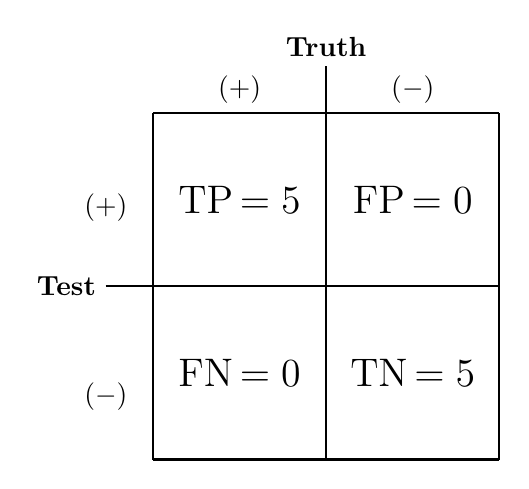
\begin{tikzpicture}[scale=2] %font=\scriptsize
    % Draw Basic Box
    \draw[thick] (0,0) -- (2.2,0);
    \draw[thick] (0,0) -- (0, 2.2);
    \draw[thick] (2.2,2.2) -- (2.2, 0);
    \draw[thick] (2.2,2.2) -- (0, 2.2);

    % Draw Box Ticks
    \draw[thick] (-0.3, 1.1) -- (2.2, 1.1);
    \draw[thick] (1.1, 0) -- (1.1, 2.5);

    % Box Labels
    % -- left side
    \coordinate[label=left:($+$)] (p1) at (-0.1,1.6);
    \coordinate[label=left:($-$)] (p2) at (-0.1,0.4);

    % -- top side
    \coordinate[label=above:($+$)] (p3) at (0.55, 2.2);
    \coordinate[label=above:($-$)] (p4) at (1.65, 2.2);

    % -- overall headers
    \coordinate[label=above:\textbf{Truth}] (p5) at (1.1, 2.5);
    \coordinate[label=left:\textbf{Test}] (p6) at (-0.3, 1.1);

    % Category Values
    \coordinate[label={\Large TP$\,=5$}] (TP) at (0.55, 1.50);
    \coordinate[label={\Large FP$\,=0$}] (FP) at (1.65, 1.50);
    \coordinate[label={\Large FN$\,=0$}] (FN) at (0.55, 0.40);
    \coordinate[label={\Large TN$\,=5$}] (TN) at (1.65, 0.40);
\end{tikzpicture}

\end{document}